% !TEX root = main.tex
\section{Time dependent amplitude fit}
\label{sec:fullFit}


%The individual amplitudes are renormalized prior to the amplitude fit such that 
%\begin{equation}
%	\int  \left\vert  \mathcal A_{i}(\phsPoint) \right\vert^{2} \, \phsd(\phsPoint) \, \dphsPoint = 1 .
%\end{equation}
%This allow us to set more intuitive starting values as the amplitude coefficients are all on a comparable scale.
%%In case of fixed lineshape parameters, the magnitude squared of the coefficients are equal to the fit fractions.
%
%In general, the signal PDF for events tagged as $\Dz \to h^+ h^- \pip \pim$ is given by
%\begin{equation}
%	\mathcal P_{\rm Sig}(\phsPoint) %= \frac{ \vert \mathcal M(X) \vert^{2} \, \phi_{4}(X) }{\int  \vert \mathcal M(X) \vert^{2} \, \phi_{4}(X) \, \text{d}X} 
%	=  
%	\frac{ [(1-w)\left\vert   A_{\Dz}(\phsPoint) \right\vert^{2} + w \, \left\vert    A_{\Dzb}(\phsPoint) \right\vert^{2} ]\,\epsilon_{\rm Sig}(\phsPoint) \, \phsd(\phsPoint) }
%	{\int [\left\vert  A_{\Dz}(\phsPoint) \right\vert^{2} + \left\vert    A_{\Dzb}(\phsPoint) \right\vert^{2} ]\, \epsilon_{\rm Sig}(\phsPoint) \, \text{d}\Phi_{4} } , 
%\label{eq:sigPDF}
%\end{equation}
%where
%$\epsilon_{\rm Sig}(\phsPoint)$ is the phase-space efficiency. 
%In the case of no $\CP$ violation, the integrals over the \Dz\ and \Dzb\ amplitudes will be equal. For the $\CP$-tagged data sets used in the $\Dz \to K^+ K^- \pip \pim$ analysis, the signal PDFs are given in Ref.~\cite{KKpipi}.
%We do not account for effects of neutral charm meson oscillations, as we expect these to be negligible in these analyses.
%
%Note that the efficiency in the numerator appears as an additive constant in the $\log {\cal L}$ that does not depend on any fit parameters such that it can be ignored.
%However, the efficiency function still enters via the normalization integrals. 
%These normalization terms are determined numerically by a MC integration technique.
%For this purpose, we use simulated events generated according to a preliminary model, pass them 
%through the full detector simulation and apply the same selection criteria as for data 
%in order to perform the MC integrals.
%For example, the first integral in \eqnPRDref{eq:sigPDF} can be approximated as 
%\begin{equation}
%	\int \left\vert   A_{\Dz}(\phsPoint) \right\vert^{2} \, \epsilon_{\rm Sig}(\phsPoint) \, \text{d}\Phi_{4}   \approx 
%	\frac{1}{N_{\rm MC}} \, \sum_{k}^{N_{\rm MC}}    \frac{\left\vert   A_{\Dz}(\bold{x_{k}}) \right\vert^{2}}
%	{\left\vert A_{\Dz}^{\prime}(\bold{x_{k}}) \right\vert^{2}}
%\end{equation}
%where $A_{\Dz}^{\prime}$ labels the preliminary amplitude model and
%$x_{k}$ is the $k$-th MC event. As a result, the efficiency can be included in the amplitude fit without explicitly modeling it.
%For $\Dz \to \pi^+ \pi^- \pip \pim$, we use a sample of $N_{\rm MC}  = 600 000$  MC events to 
%ensure that the uncertainty on the integral is less than $0.5 \%$.

\subsection{Signal Model Construction}
\label{sec:LASSO}

The light meson spectrum comprises multiple resonances which are expected to contribute to $B_s \to D_s K \pi \pi$  decays as intermediate states. 
Apart from clear contributions coming from resonances such as $K_{1}(1270)$, $K_{1}(1400)$ $\rho(770)$ and $K^*(892)^0$, 
the remaining structure is impossible to infer due to
the cornucopia of broad, overlapping and interfering resonances 
within the phase space boundary.
The complete list of considered amplitudes can be found in Appendix \ref{a:decays}.

To build the amplitude model, one could successively add amplitudes on top of one another until a reasonable agreement between data and fit was achieved.
However, this step-wise approach is not particularly suitable for amplitude analyses as discussed in Ref.~\cite{Guegan:2015mea}.
%In practice, this sum has to be truncated at some point.
%It is clear that adding more fit parameters will 
%describe our data better
%but including too many degrees of freedom leads to overfitting,
%\ie reduces predictive power and
Instead, we include the whole pool of amplitudes in the first instance and use the 
Least Absolute Shrinkage and Selection Operator~\cite{Tibshirani94regressionshrinkage,Guegan:2015mea} (LASSO) approach to limit the model complexity.
%, as proposed in Ref.~\cite{Guegan:2015mea}. 
% in the context of amplitude analyses.
In this method, the event likelihood is extended by a penalty term
\begin{equation}
	-2 \, \log \mathcal L \to -2 \, \log \mathcal L + \lambda \, \sum_{i} \sqrt{ \int \vert a_{i} \, A_{i}(\phsPoint) \vert^{2} \, \text{d}\Phi_{4}  },
\end{equation}
which 
%regularizes the amplitude coefficients.
%The imposed constraint on the 
%which limits the model complexity. 
% penalizing the absolute values of the
%coecients introduces shrinkage towards zero
%This constrained optimization 
shrinks the amplitude coefficients
%estimated parameters 
towards zero.
The amount of shrinkage is controlled by the parameter $\lambda$, to be tuned on data.
Higher values for $\lambda$ encourage sparse models, \ie models with only a few non-zero amplitude coefficients.
%Scanning over possible $\lambda$ values results in a ensemble of models with different 
The optimal value for $\lambda$ is found by minimizing the Bayesian information criteria~\cite{BIC} (BIC),
\begin{equation}
	\text{BIC}(\lambda) = - 2 \, \log \mathcal L + r  \, \log N_{\rm Sig},
\end{equation}
where $N_{\rm Sig}$ is the number of signal events and $r$ is the number of amplitudes with a decay fraction above 
a certain threshold.
In this way, the optimal $\lambda$ balances
the fit quality ($- 2 \, \log  \mathcal L$) against the model complexity.
The LASSO penalty term is only used to select the model. 
Afterwards, this term must be discarded in the final amplitude fit with the selected model, otherwise the parameter uncertainties would be biased. 

The set of amplitudes is selected using the optimal value of $\lambda=28$, and is henceforth called the LASSO model; 
Figure \ref{fig:BIC}(a) shows the distribution of BIC values obtained by scanning over $\lambda$
where we choose the decay fraction threshold to be $0.5 \%$.
%It is important to note that there are certain groups of amplitudes with the same angular distribution 
%that are prone to produce artificially high interference effects.
%Amongst them are the di-scalar amplitudes: 
%$D \to (\pi \, \pi)_{S} \, (\pi \, \pi)_{S}$, $D \to (\pi \, \pi)_{S} \, \sigma$, $D \to \sigma \, \sigma$, $D \to \sigma \, f_{0}(1370)$
%and $D \to f_{0}(1370) \, f_{0}(1370)$
%as well as the di-vector amplitudes:  $D \to (\pi \, \pi)_{P} \, (\pi \, \pi)_{P}$, $D \to (\pi \, \pi)_{P} \, \rho(1450)^{0}$ and $D \to \rho(1450)^{0} \, \rho(1450)^{0}$.
%In these cases, only one amplitude of the group is included at a time and the model selection is performed for each choice.
In addition, we repeated the model selection procedure under multiple different conditions:
\begin{enumerate}
	\item The fit fraction threshold for inclusion in the final model was varied within the interval $[0.05, 5] \%$.
		The set of selected amplitudes is stable for thresholds between $0.1\%$ and $1\%$. 
		Other choices result in marginally different models containing one component more or less.
	\item Instead of BIC, the Akaike information criteria ($\text{AIC}(\lambda) = -2 \, \log  \mathcal L + 2 \, r$ \cite{AIC}) was used to optimize $\lambda$.
		For a given threshold, the AIC method tends to prefer %slightly 
		lower $\lambda$ values.
		However, the set of models obtained varying the threshold within the interval $[0.05, 5] \%$
		is identical to the BIC method. 
	\item The amplitudes selected under nominal conditions were excluded one-by-one from the set of all amplitudes considered.  
\end{enumerate}
From that we obtained a set of alternative models shown in Appendix~\ref{a:alternative}.

%Due to the vast number of potential amplitude components and computational limits imposed by the consideration of multiple data samples in the $\Dz \to \KKpipi$ analysis, a staged LASSO method using only the flavor-tagged data, 
%representing over 90\% of the available statistics, is employed. The approach taken is based on the assumption that the signal decay proceeds primarily by doubly resonant decays, \ie cascade and quasi-two-body decays, rather than decay amplitudes with non-resonant components. In Stage 1, only doubly resonant decays along with the simplest non-resonant component $(K^+K^-)_{S} \, (\pi^+ \pi^-)_{S}$ are considered. Figure \ref{fig:BIC}(b) shows a plot of the complexity factor $\lambda$, against the resulting BIC values. We found that the fit cannot distinguish between amplitudes with $K^*(1680)^+ \to K^*(892)^0\, \pip$ and $K^*(1410)^+ \to K^*(892)^0 \, \pip$, which both peak outside the kinematic range of the \D\ decay's phase space. We therefore only include $K^*(1680)^+ \to K^*(892)^0\, \pip$ in our nominal model. An alternative fit with the $K^*(1410)^{+}$, which has marginally worse fit quality is presented in Table~\ref{tab:alternativeModels2}.
%
%In Stage 2, the LASSO procedure is again performed with the components selected by Stage 1 and all single-resonant components. It should be noted in the case of 
%%flavor-non-specific 
%cascade decays that if LASSO picked an amplitude component but not its conjugate decay in the first stage, the conjugate is also considered again in this stage. Once more, the interplay between $D \rightarrow SS$ amplitudes leads to very large interference terms, and thus $f_0(980) \,(\pi^+ \pi^-)_{S}$ and $f_0(980) \, (K^+ K^-)_{S}$ components are considered as a replacement for the non-resonant $(K^+K^-)_{S} \, (\pi^+ \pi^-)_{S}$ component in an alternative model. 
% %Similar interplay is seen between $\phi(1020) \rho^0(770)$ and $\phi(1020) (\pi^+ \pi^-)_{P}$, both in a relative $P$-wave.
%%With the exception of $\phi(1020) (\pi^+ \pi^-)_{P}$ in a relative $P$-wave, only non-resonant $S$-waves combined with vector components are selected, however the component $\phi(1020) \rho^0(770)~P~$-wave drops out. The decays $\phi(1020) \{ \pi^+ \pi^- \}_{P}$ in a relative $P$-wave and $\phi(1020) \rho^0(770)~P~$-wave share the same angular structure and so given the initial assumption $\phi(1020) \rho^0(770)~P~$-wave is selected.
%The final fit merges the components chosen in Stage 1 and Stage 2 and includes the \CP-tagged data. Within this set of amplitudes, 6 are considered insignificant relative to their error and removed from the fit with no significant impact on fit quality.

%\begin{figure}[b]
%  \centering
%  \includegraphics[width=0.49\textwidth, height=!]{figs/BIC_4pi.eps} 
%  \includegraphics[width=0.49\linewidth, height=!]{figs/BIC_KKpipi.eps}
%  \caption{Difference in the BIC value from its minimum as function of the LASSO parameter $\lambda$ for $\Dz \to \fourpi$ (a) and Stage 1 $\Dz \to \KKpipi$ (b).}
%  \label{fig:BIC}
%\end{figure}


\subsection{Results}

\begin{table}[h]
\centering
\caption{Result of the phase-space integrated fit to $B_s \to D_s K \pi \pi$ data.}
\begin{tabular}{c c c}
\hline
\hline
& Fit parameter & Value \\
\hline
& $C$ &  xx.xx  $\pm$ 0.126\\
&$D$ &  xx.xx  $\pm$ 0.386\\
&$\bar D$ &  xx.xx  $\pm$ 0.360\\
& $S$ &  xx.xx  $\pm$ 0.177\\
& $\bar S$ &  xx.xx  $\pm$ 0.169\\
\hline
\hline
\end{tabular}
\label{table:timeFit_signal}
\end{table}


\begin{tabular}{l r}
\hline
\hline
Decay channel & Fraction [$\%$] \\
\hline
$B_s \to K(1)(1270)^+( \to K^*(892)^0( \to K^+ \, \pi^-) \, \pi^+) \, D_s^-$ & 5.88 $\pm$ 17.30 \\
$B_s \to K(1)(1270)^+( \to K(0)^*(1430)^0( \to K^+ \, \pi^-) \, \pi^+) \, D_s^-$ & 4.07 $\pm$ 0.90 \\
$B_s \to K(1)(1270)^+( \to \rho(770)^0( \to \pi^+ \, \pi^-) \, K^+) \, D_s^-$ & 9.40 $\pm$ 1.75 \\
$B_s \to K(1)(1400)^+( \to K^*(892)^0( \to K^+ \, \pi^-) \, \pi^+) \, D_s^-$ & 53.87 $\pm$ 10.03 \\
$B_s \to K^*(1410)^+( \to K^*(892)^0( \to K^+ \, \pi^-) \, \pi^+) \, D_s^-$ & 16.88 $\pm$ 3.14 \\
$B_s \to K^*(1410)^+( \to \rho(770)^0( \to \pi^+ \, \pi^-) \, K^+) \, D_s^-$ & 7.55 $\pm$ 1.57 \\
$B_s \to ( D_s^- \, \pi^+)_{P} \, K^*(892)^0( \to K^+ \, \pi^-)$ & 6.97 $\pm$ 1.30 \\
 \hline
 Sum & 104.61 $\pm$ 5.23 \\
\hline
\hline
\end{tabular}

\begin{tabular}{l r}
\hline
\hline
Decay channel & Fraction [$\%$] \\
\hline
$B_s \to K(1)(1270)^+( \to K^*(892)^0( \to K^+ \, \pi^-) \, \pi^+) \, D_s^-$ & 16.69 $\pm$ 20.48 \\
$B_s \to K(1)(1270)^+( \to K(0)^*(1430)^0( \to K^+ \, \pi^-) \, \pi^+) \, D_s^-$ & 11.57 $\pm$ 2.24 \\
$B_s \to K(1)(1270)^+( \to \rho(770)^0( \to \pi^+ \, \pi^-) \, K^+) \, D_s^-$ & 26.72 $\pm$ 4.19 \\
$B_s \to K(1)(1400)^+( \to K^*(892)^0( \to K^+ \, \pi^-) \, \pi^+) \, D_s^-$ & 16.02 $\pm$ 2.51 \\
$B_s \to K(1460)^+( \to K^*(892)^0( \to K^+ \, \pi^-) \, \pi^+) \, D_s^-$ & 20.47 $\pm$ 3.21 \\
$B_s \to ( D_s^- \, \pi^+)_{P} \, K^*(892)^0( \to K^+ \, \pi^-)$ & 32.76 $\pm$ 5.14 \\
$B_s \to ( D_s^- \, K^+)_{P} \, \rho(770)^0( \to \pi^+ \, \pi^-)$ & 10.04 $\pm$ 1.57 \\
 \hline
 Sum & 134.26 $\pm$ 5.97 \\
\hline
\hline
\end{tabular}



\begin{figure}[h]
	\centering
		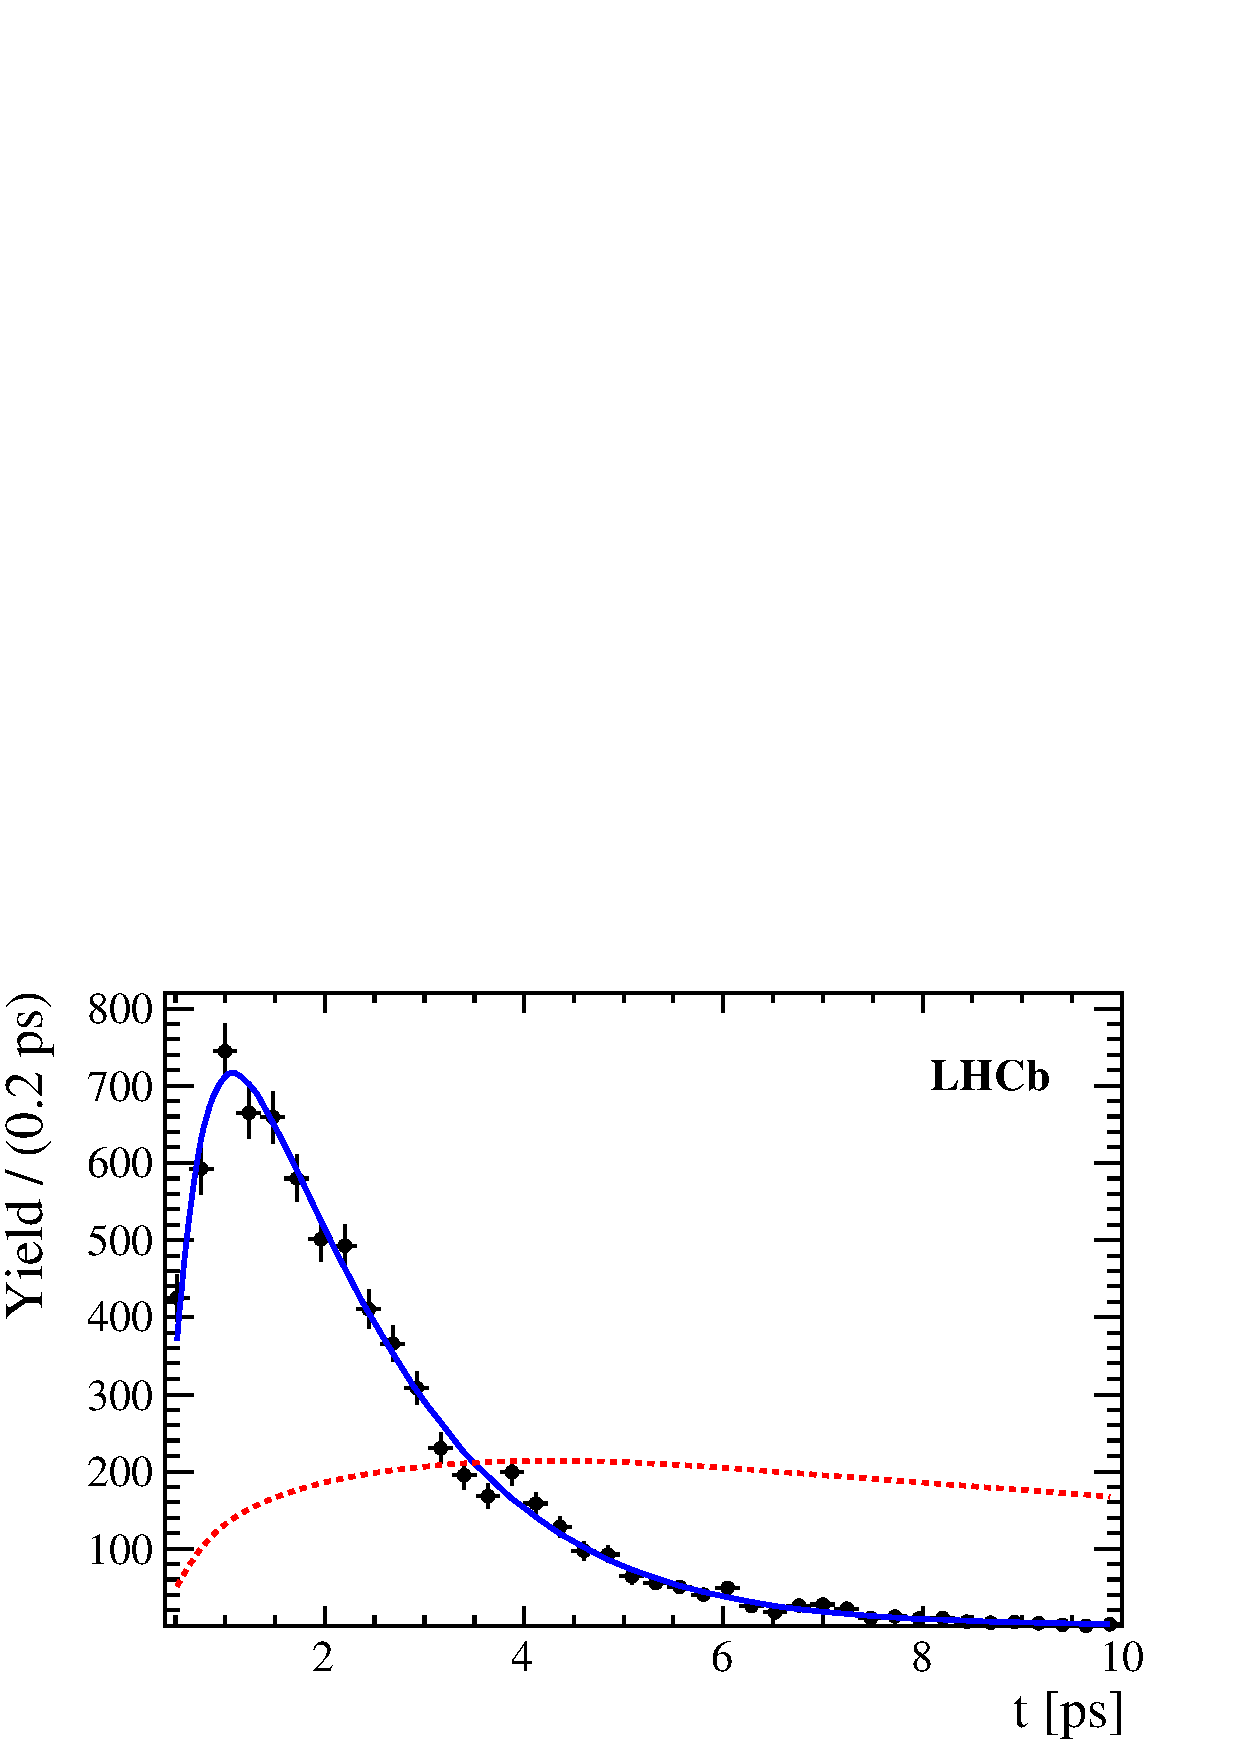
\includegraphics[width=0.3\textwidth, height = !]{figs/fullFit/signal/h_t.pdf} 
		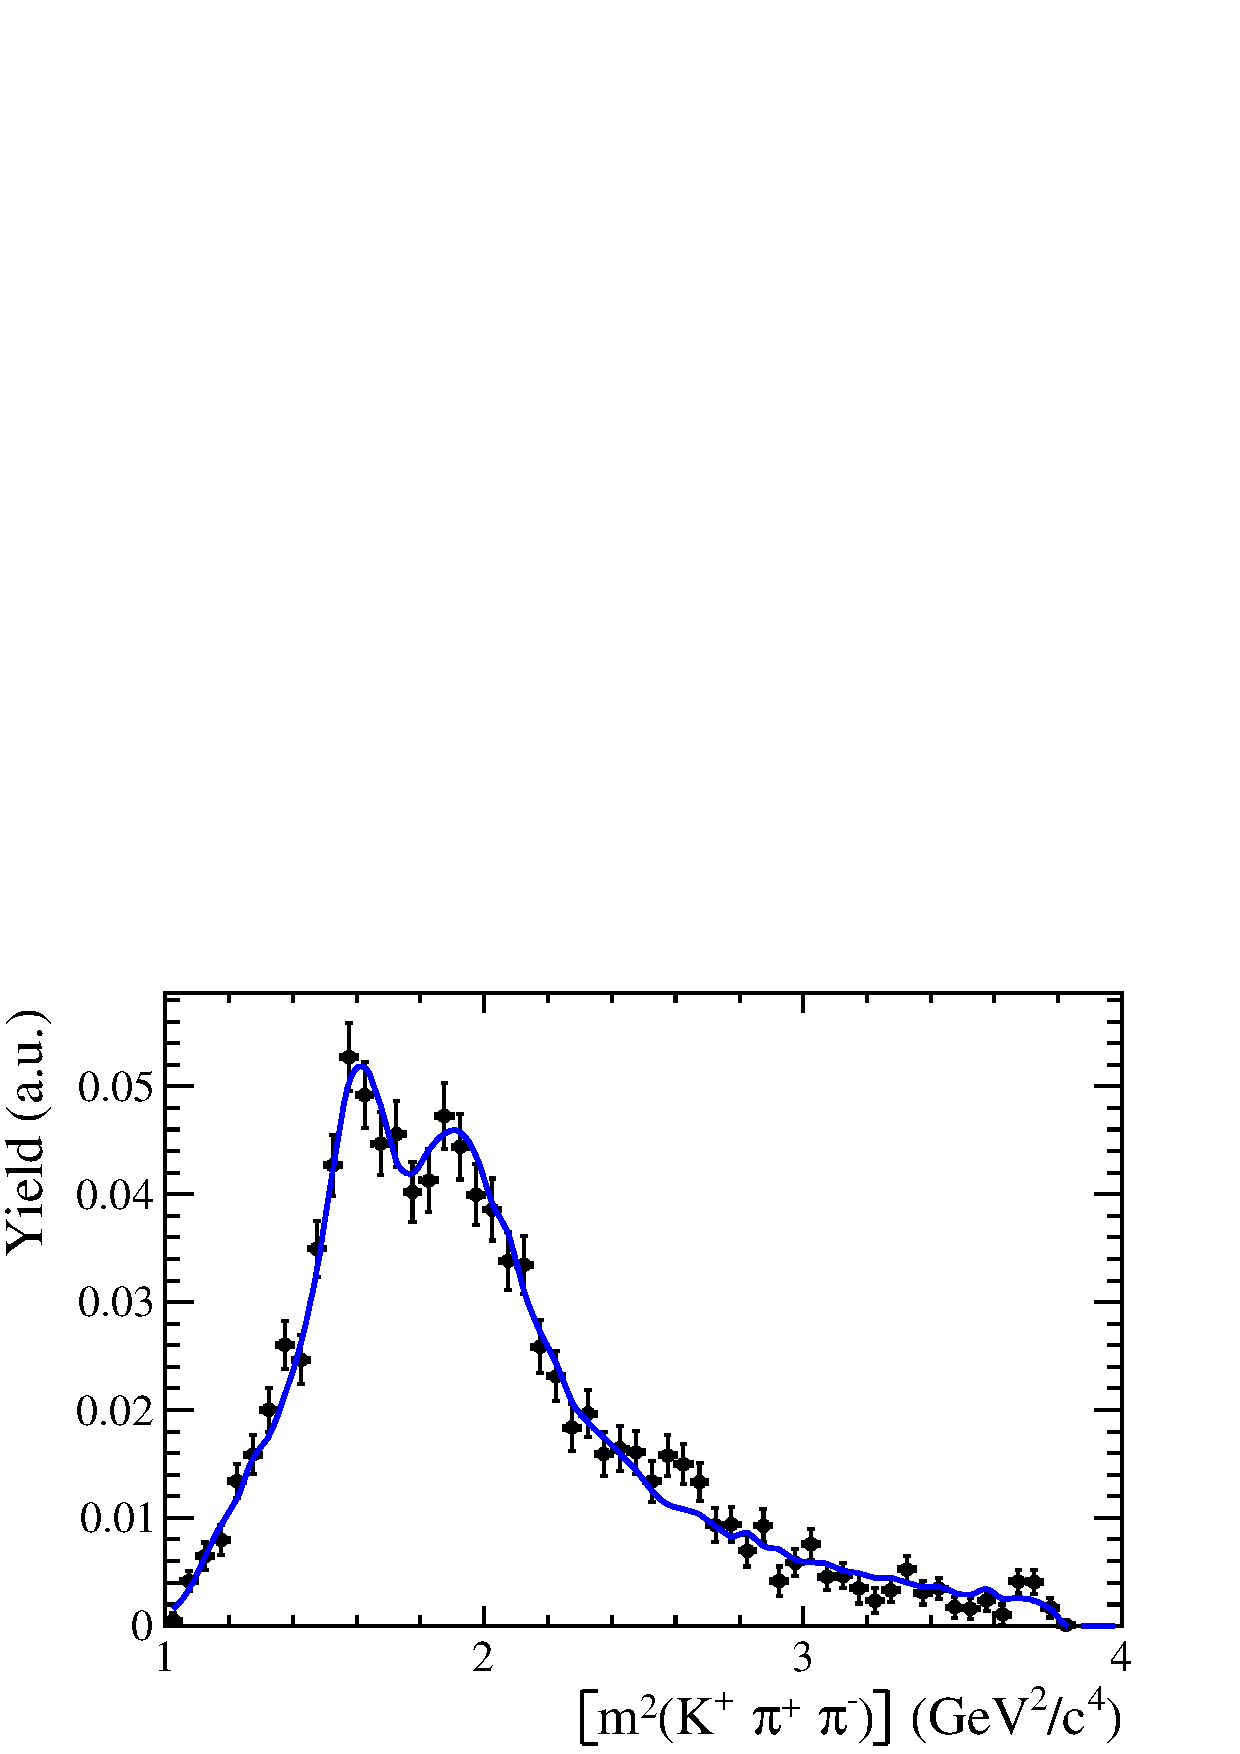
\includegraphics[width=0.3\textwidth, height = !]{figs/fullFit/signal/s_Kpipi.pdf} 
		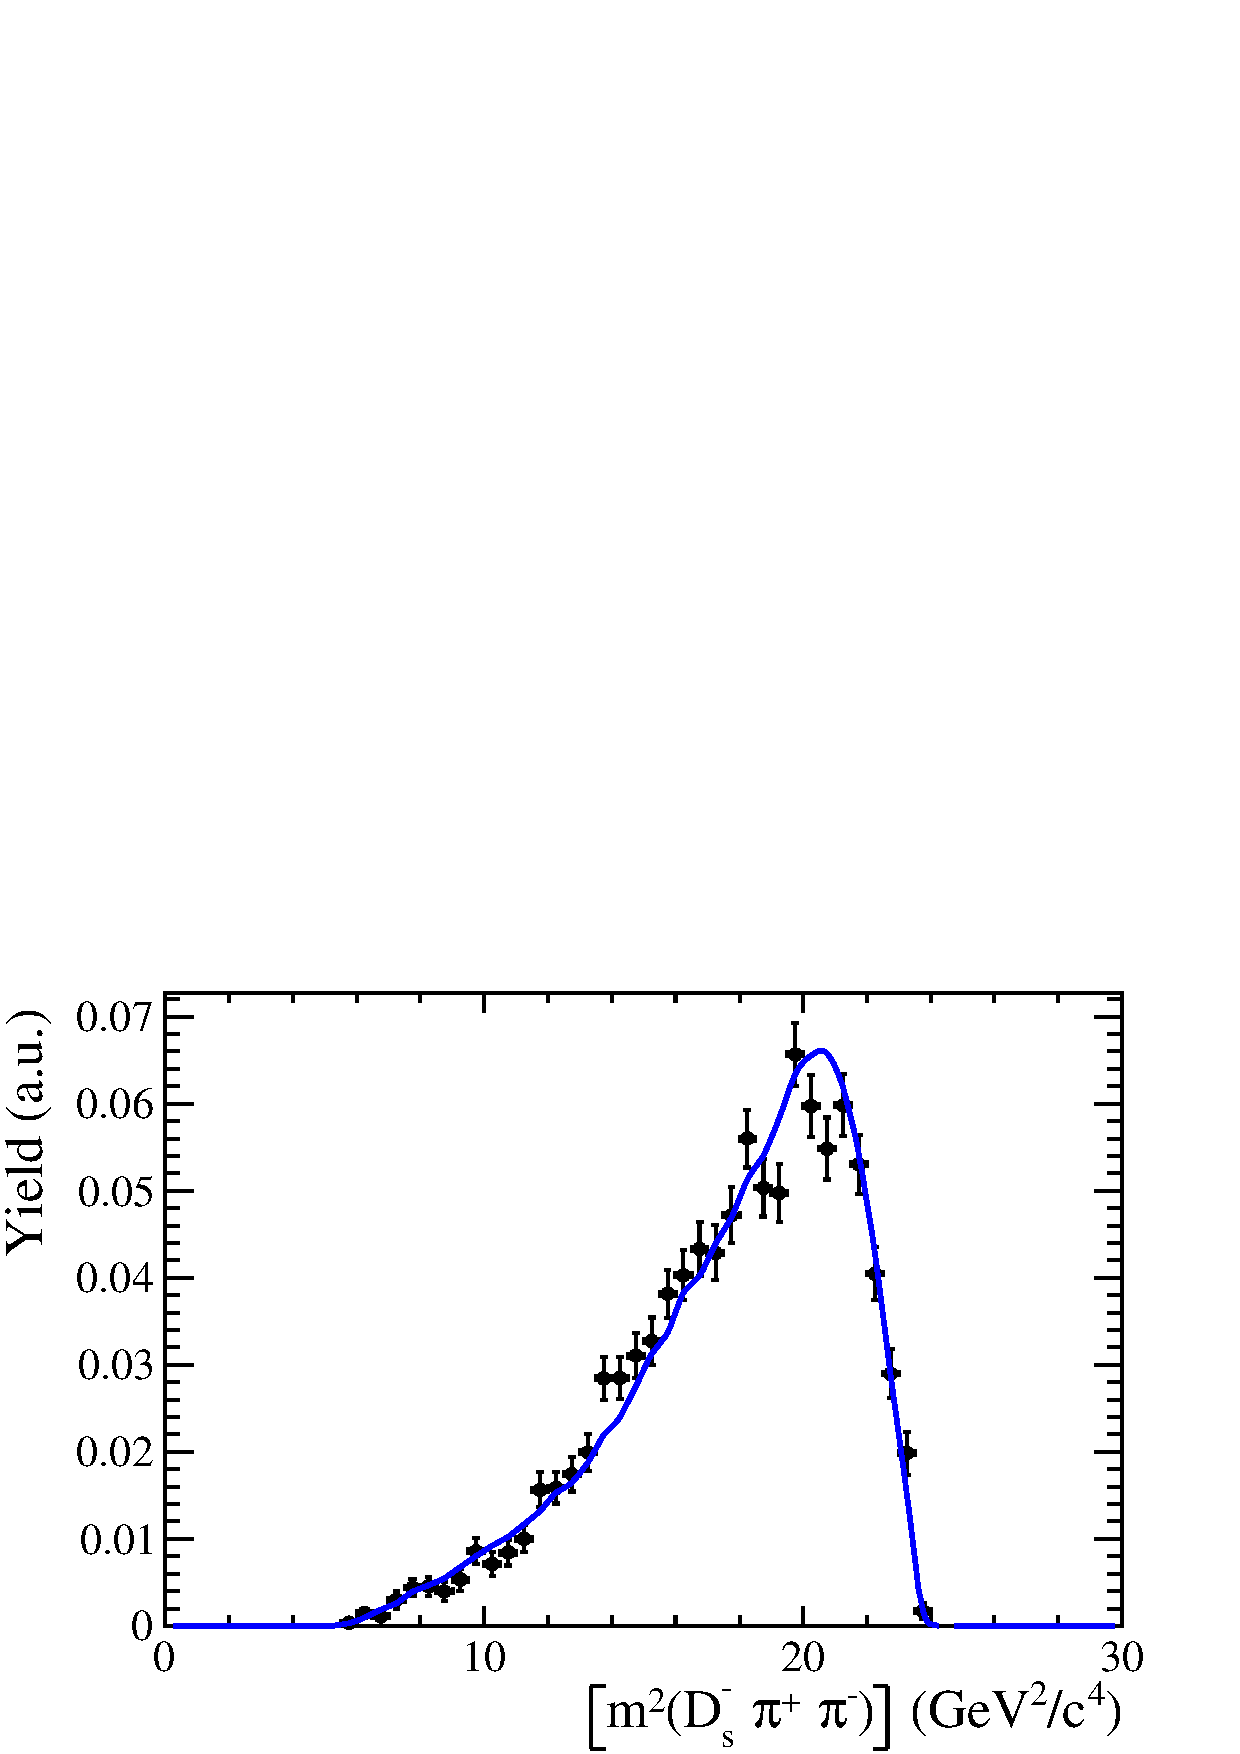
\includegraphics[width=0.3\textwidth, height = !]{figs/fullFit/signal/s_Dspipi.pdf} 

		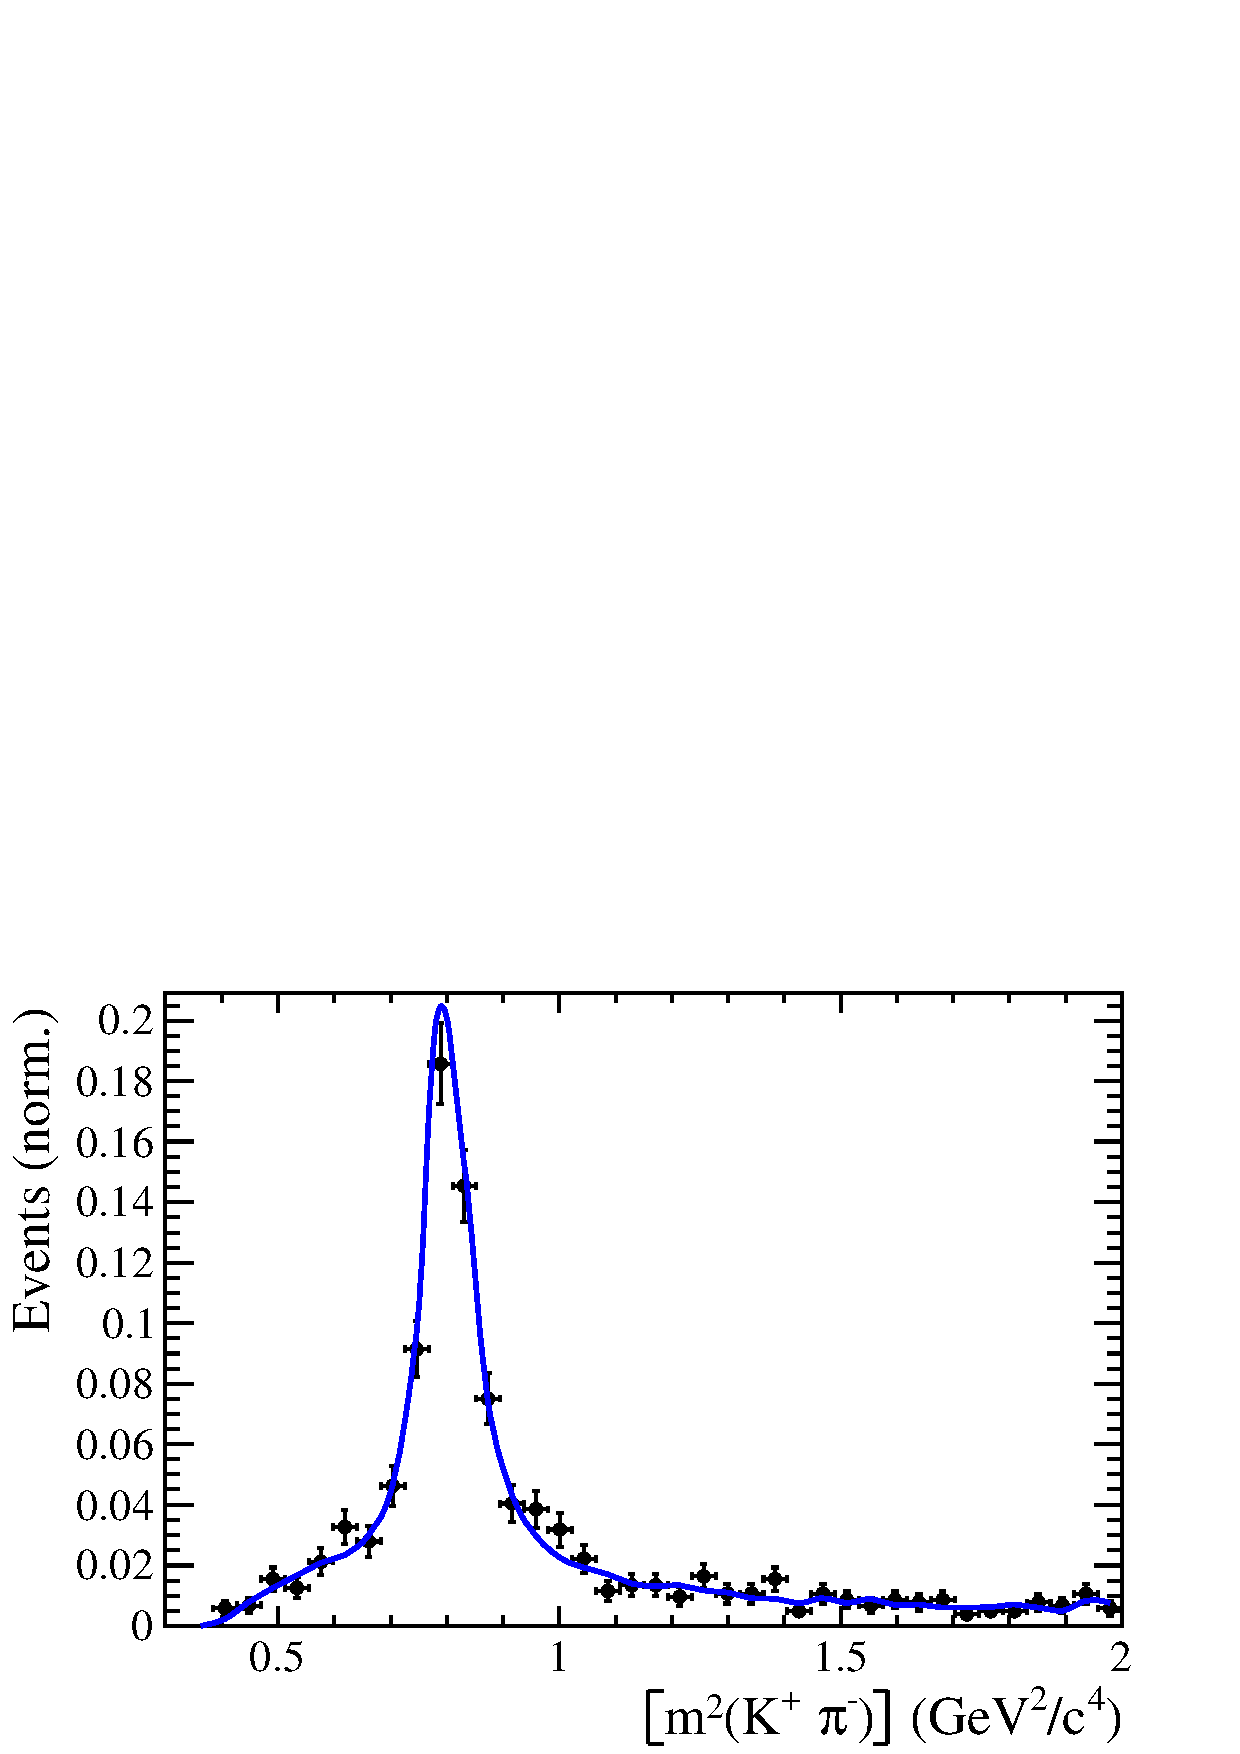
\includegraphics[width=0.3\textwidth, height = !]{figs/fullFit/signal/s_Kpi.pdf} 
		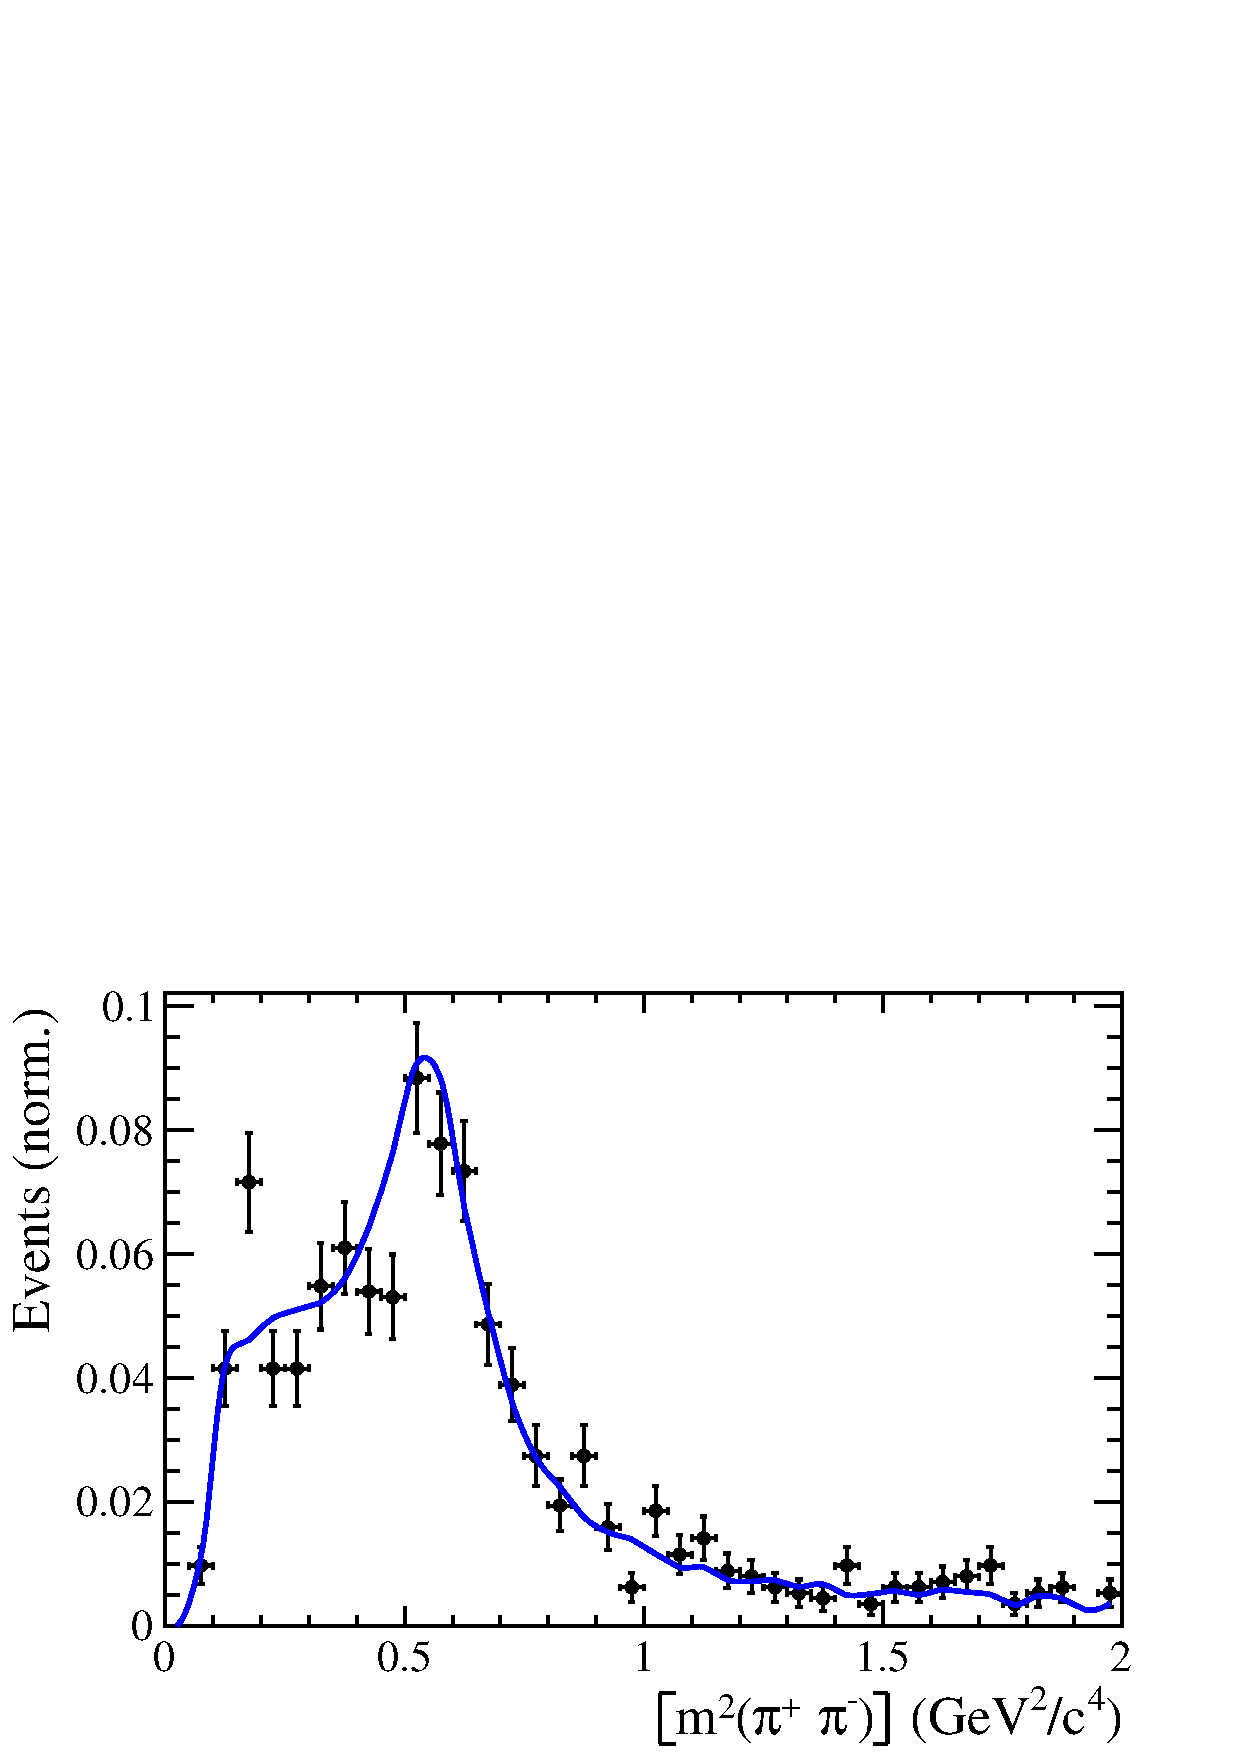
\includegraphics[width=0.3\textwidth, height = !]{figs/fullFit/signal/s_pipi.pdf} 
		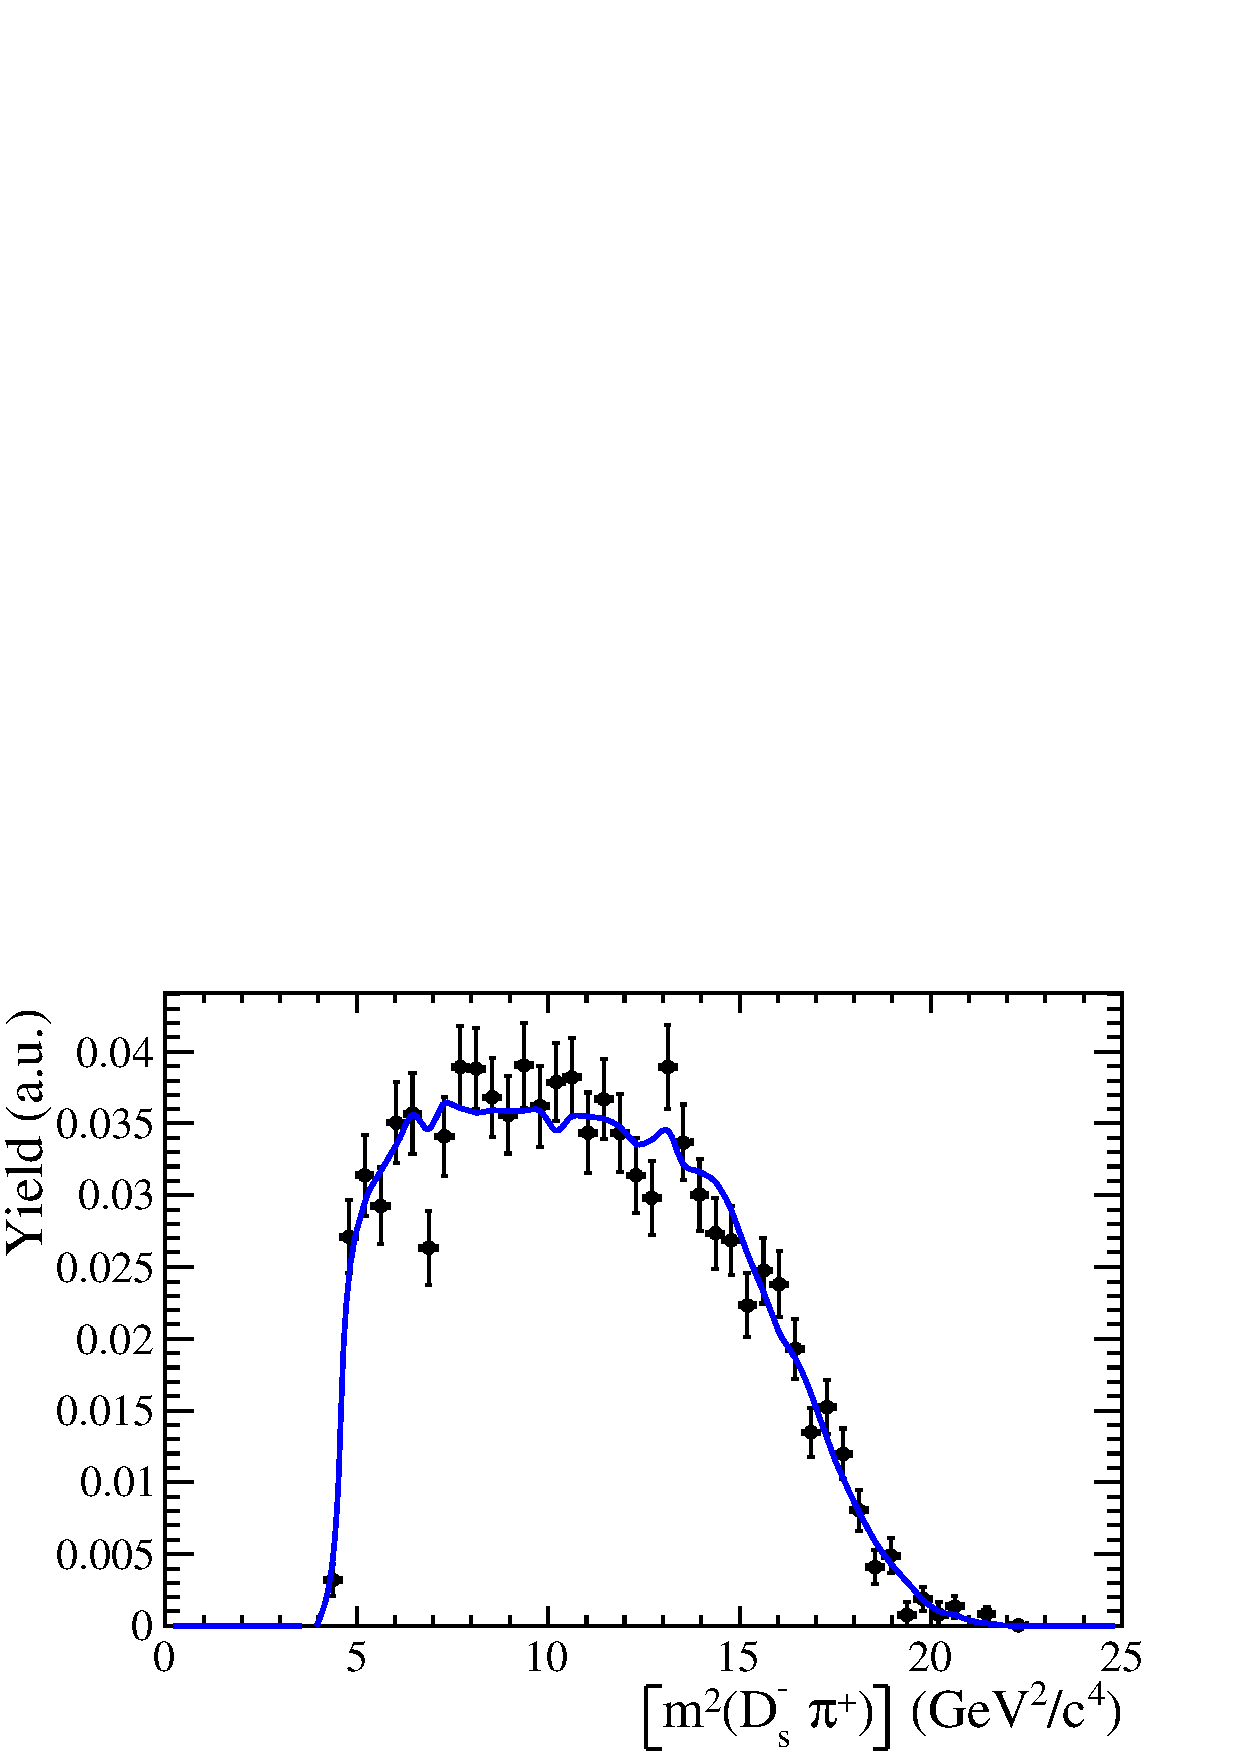
\includegraphics[width=0.3\textwidth, height = !]{figs/fullFit/signal/s_Dspi.pdf} 

		\caption{} 		
\end{figure}	